\documentclass{article}
\usepackage[a4paper]{geometry}
\usepackage[spanish]{babel}
\usepackage{parskip}
\usepackage{setspace}
\usepackage{graphicx}
\usepackage{fancyhdr}
\usepackage{typearea}
\geometry{total={6in, 9in}}
\usepackage{blindtext} % no sé 
\usepackage{makeidx} % no sé 
\usepackage{lscape}
\usepackage{pdflscape}
\usepackage{fancyhdr}
\usepackage{pdfpages}
\usepackage{rotating}
\usepackage{etoolbox}
\usepackage[absolute]{textpos}
\usepackage{listings}

\lstdefinestyle{customc}{
  language=C++,
  showstringspaces=false,
  basicstyle=\footnotesize\ttfamily,
  keywordstyle=\bfseries\color{green!40!black},
  commentstyle=\itshape\color{purple!40!black},
  identifierstyle=\color{blue},
  stringstyle=\color{orange},
}

\lstset{escapechar=@,style=customc}

\newcommand{\tabitem}{%
  	\usebeamertemplate{itemize item}\hspace*{\labelsep}}
\usepackage[hidelinks]{hyperref}

%HEADRULE

\pagestyle{fancy}
\setlength{\headheight}{30.2pt}
\setlength{\headsep}{30pt}
% INICIO DE PÁGINAS
\begin{document}
\begin{titlepage}
	
	
	\begin{center}
		{\LARGE \textbf{UNIVERSIDAD NACIONAL DE INGENIERÍA}}\\
		\vspace{5 mm}
		{\large \textbf{Facultad de Ingeniería Industrial y de Sistemas}}\\
		\vspace{15.5 mm}
		\begin{figure}[h]
			\centering 
			
\includegraphics[width=0.45\textwidth]{images/CiberSecFIIS.png}
		\end{figure}
		\vspace{4 mm}	
		{\Large \textbf{Informes de exploración de vulnerabilidades en HTB} }\\
		\vspace{5 mm}
		
		\onehalfspacing  % Espaciamiento 1.5
		{\Large \textbf{``{\@De las máquinas: OpenAdmin, Fuse \\Magic, Remote }''} }\\
		
		\singlespacing  % Fin del espaciamiento 1.5
		
		\vspace{4 mm}	

		\vspace{20 mm}
		{\large \textbf{ELABORADO POR:} }\\
		\vspace{10 mm}
		\begin{center}
			\begin{minipage}{0.7\textwidth}
			  \begin{itemize}
				\item \Large Alfonso Suárez, Luis
				\item \Large Mottoccanche Tantaruna, Joseph
				\item \Large Chi Jon, Lau
			  \end{itemize}
			\end{minipage}
		  \end{center}

		\vspace{5 mm}	
	\end{center}

\end{titlepage}


\clearpage
\tableofcontents
\clearpage
% ----------------------------OPENADMIN-----------------------------------
\section{OpenAdmin}
\subsection{Reconocimiento}
\subsection{Escaneo de Vulnerabilidades}
\subsection{Enumeración}
\subsection{Explotación}
\subsection{Post Explotación}


\clearpage
% ----------------------------REMOTE-----------------------------------
\section{Remote}
\subsection{Reconocimiento}
Lo primero a hacer en este caso es un escaneo de nmap, para encontrar algunos puertos abiertos y servicios corriendo, en este caso se encontraron los puertos 21, 80 y 445 abiertos principalmente.

\begin{figure}[h]
	\center
	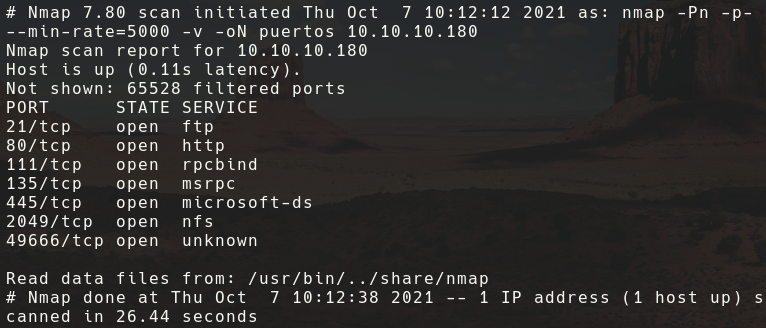
\includegraphics[width=0.8\textwidth]{images/remote/nmap_remote.png}
	\caption{nmap remote}
\end{figure}
 
\subsection{Escaneo de Vulnerabilidades}

Como primer escaneo de vulnerabilidades se intenta con el mismo nmap, con la opción "--script vuln", esto probará as vulnerabilidades más comunes en el server.

\begin{figure}[h]
	\center
	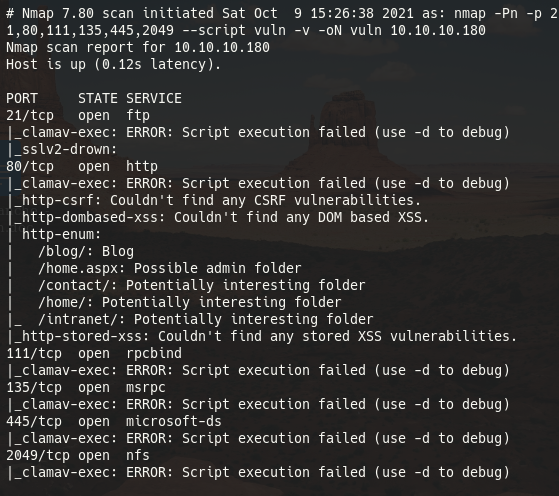
\includegraphics[width=0.7\textwidth]{images/remote/nmap_vuln.png}
	\caption{vulnerabilidades por nmap}
\end{figure}
\subsection{Enumeración}

Luego de ver los puertos, nmap no nos bota una vulnerabilidad por FTP, pero de todos modos nunca está de más probar si encontramos algo, sin embargo en esta ocasión no encontramos nada relevante.
\begin{figure}[h]
	\center 
	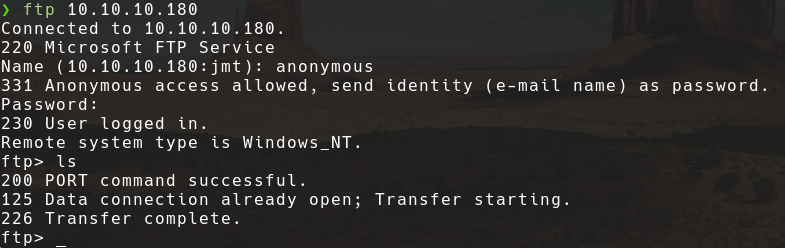
\includegraphics[width=0.95\textwidth]{images/remote/ftp.png}
	\caption{logueo anónimo por FTP}
\end{figure}

Intentamos luego con la página ubicada en el puerto 80, a ver si encontramos algo, y efectivamente encontramos una página que tiene diferentes apartados para revisar, buscamos info en los cuadros y en toda la página pero es solo texto generado de relleno, así que no hay información relevante en estas páginas para diccionarios.
\begin{figure}[h]
	\center 
	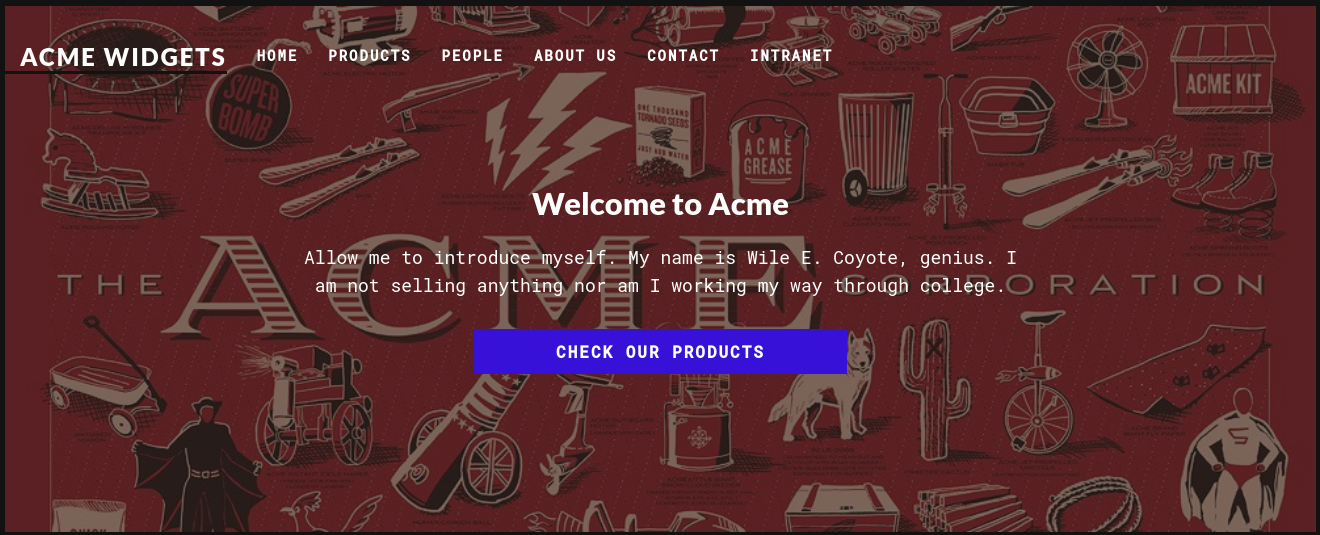
\includegraphics[width=0.95\textwidth]{images/remote/index_pagina.png}
	\caption{logueo anónimo por FTP}
\end{figure}

\clearpage

Entre todas las páginas encontramos un apartado de login, está en el mismo servidor así que se ve bastante interesante junto a que el framework es de umbraco según el wappalizer.
\begin{figure}[h]
	\center 
	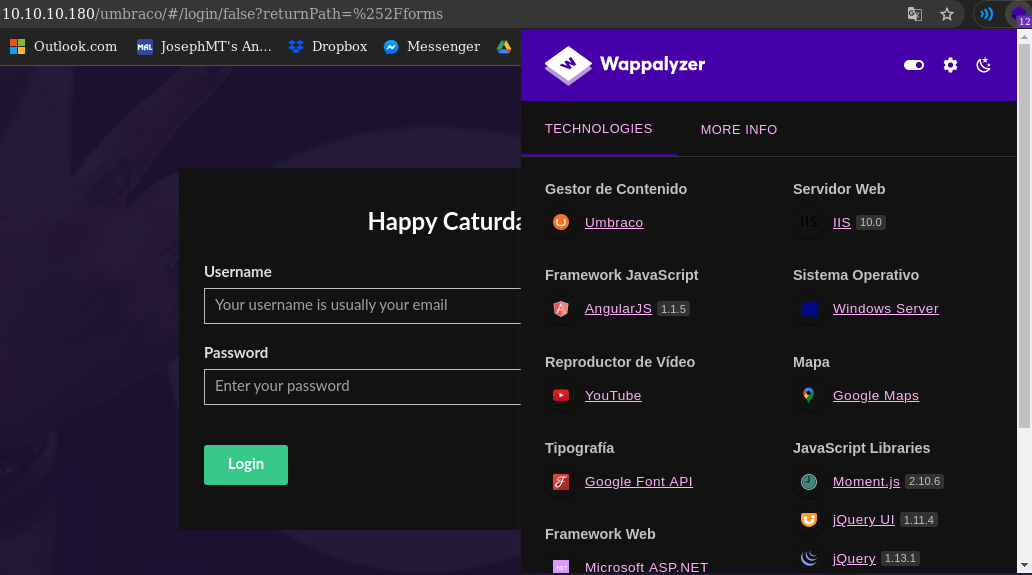
\includegraphics[width=0.85\textwidth]{images/remote/wappalizer.png}
	\caption{Resultados de wappalizer}
\end{figure}

Intentamos un escaneo con dirb para escanear los posibles directorios ocultos, donde se encontraron muchos directorios que de forma normal hubieran sido localizados y otros que hacen referencia a redirecciones, algunos que mostraron un error de configuración pero no grave.
\begin{figure}[h]
	\center 
	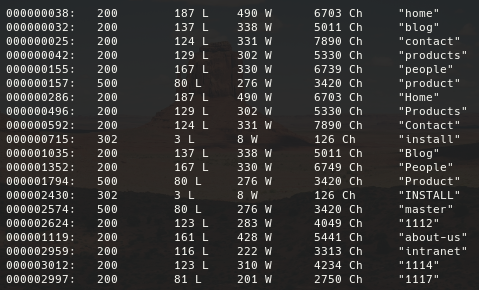
\includegraphics[width=0.85\textwidth]{images/remote/dirb.png}
	\caption{Escaneo con la herramienta dirb}
\end{figure}

\clearpage

Luego para tratar de buscar por los archivos compartidos se usa el comando llamado showmonts, que viene en la herramienta nfs-common.
\begin{figure}[h]
	\center 
	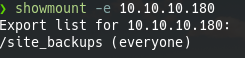
\includegraphics[width=0.6\textwidth]{images/remote/nfs.png}
	\caption{Obtención del backup}
\end{figure}

Luego creando una carpeta para guardar el contenido extraído con el comando "mount -t nfs 10.10.10.180:/site\_backups".
\\ una vez copiado esto tenemos carpetas interesantes, nuestro objetivo parecen ser credenciales de la base de datos para por medio de esas acceder al servidor original, entonces primero buscamos un poco.
\begin{figure}[h]
	\center 
	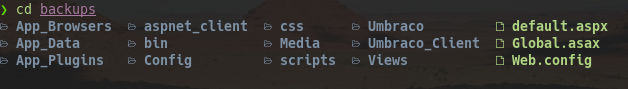
\includegraphics[width=0.95\textwidth]{images/remote/backup.png}
	\caption{Revisado del backup}
\end{figure}
Entonces encontramos una password en hash dentro de "App\_Data/Umbraco.sdf"
La obtuvimos mediante el comando strings probando en diferentes archivos de configuración grepeando pass, luego de encontrarla en esta ruta vimos que grepeando pass no nos daba mucha información adicional al correo de login, así que probamos otro filtro.
\begin{figure}[h]
	\center 
	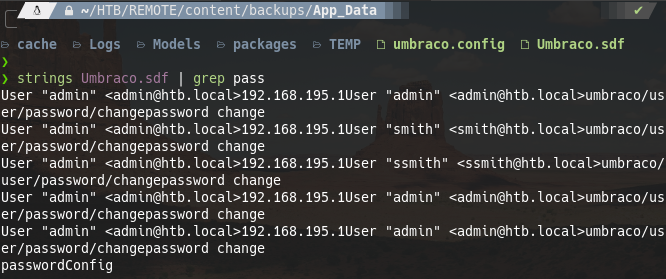
\includegraphics[width=0.95\textwidth]{images/remote/strings_pass.png}
	\caption{Encontrando el fichero con la contraseña}
\end{figure}

\clearpage

Entonces probando el filtro "admin" en base a los resultados anteriors, y encontramos un hash, el cual mediante hash-identifier pudimos comprobar su naturaleza SHA1.
\begin{figure}[h]
	\center 
	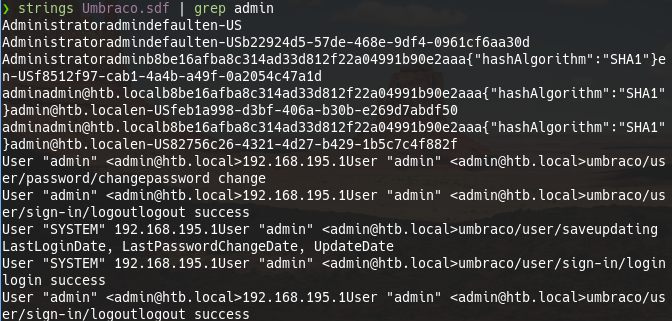
\includegraphics[width=\textwidth]{images/remote/strings_admin.png}
	\caption{Encontrando la contraseña cifrada}
\end{figure}

Ahora posteriormente lo que sigue es intentar el crackeo de esta contraseña cifrada en SHA1, para nuestra suerte este tipo de cifrado es completamente obsoleto al poseer posiblidad de colisiones en su algoritmo.
Por lo cual en diferentes sitios online se pueden encontrar formas de crackear la contraseña, y el resultado es la obtención de la contraseña "baconandcheese".
\begin{figure}[h]
	\center 
	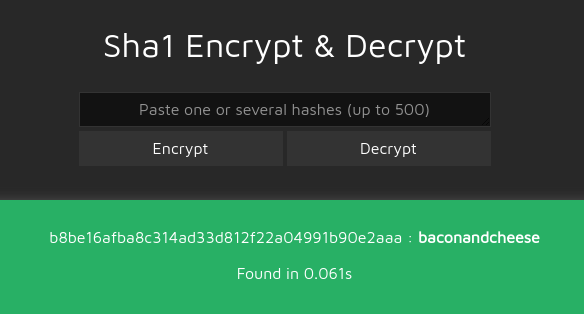
\includegraphics[width=0.95\textwidth]{images/remote/sha1.png}
	\caption{Encontrando la contraseña en texto claro}
\end{figure}

\clearpage

Probando ya tenemos acceso a la página de administrador dentro de la página, donde se permite el subido de imágenes, lo cual nos hace dar una idea de una posible inyección o ejecución remota de comandos, para lo cual primero buscaremos si existe algún exploit que aproveche esta vulerabilidad en github.
\begin{figure}[h]
	\center 
	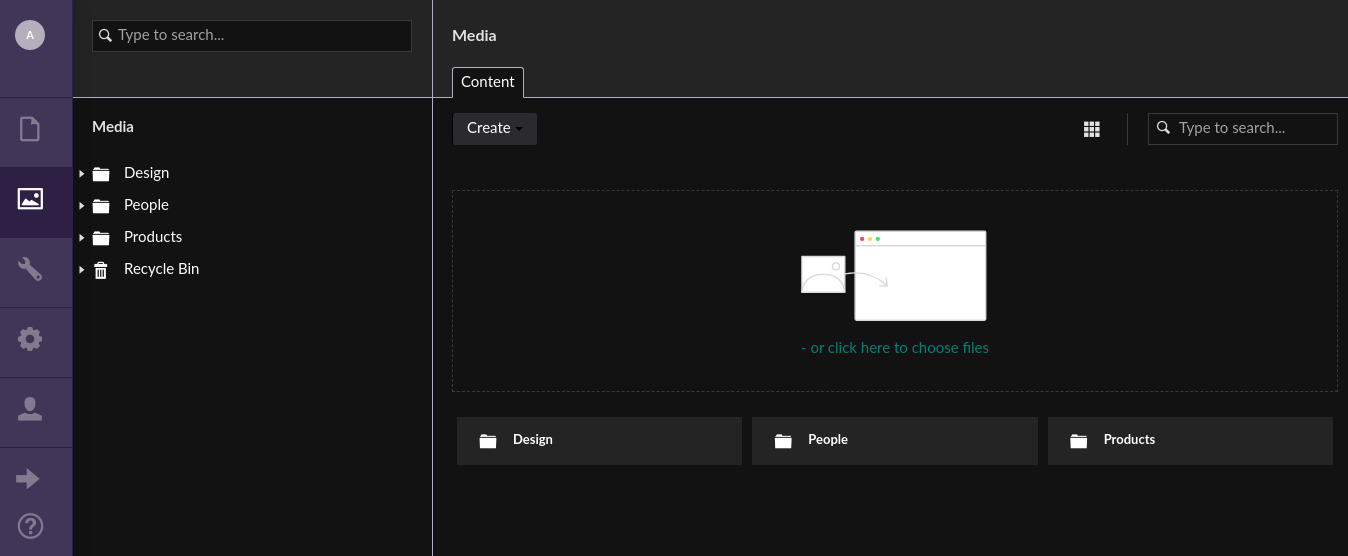
\includegraphics[width=\textwidth]{images/remote/admin-panel.png}
	\caption{Encontrando la contraseña en texto claro}
\end{figure}


\subsection{Explotación}
\subsubsection{Obtención de Acceso como usuario}
Entonces comenzamos con la búsqueda del script en github, para lo cual nos encontramos el siguiente. \textbf{\href{https://github.com/noraj/Umbraco-RCE}{https://github.com/noraj/Umbraco-RCE}}
Descargando el exploit y ejecutándolo obtenemos una ejecución remota de comandos mediante powershell.
\begin{figure}[h]
	\center 
	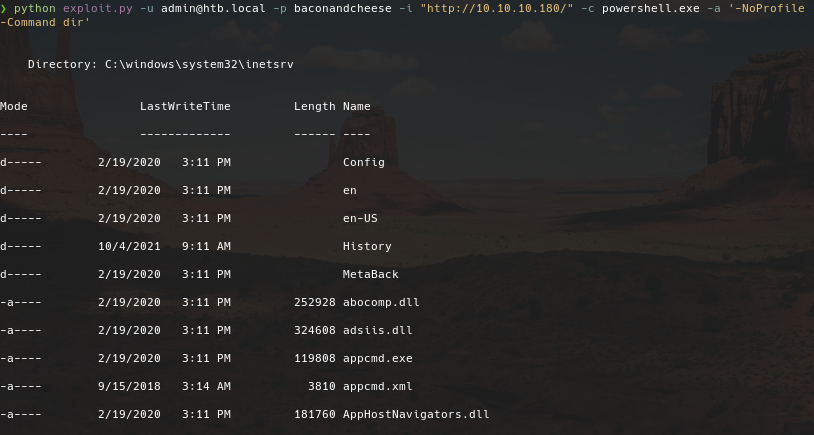
\includegraphics[width=\textwidth]{images/remote/script-1.png}
	\caption{Probando Ejecución Remota de Comandos}
\end{figure}

\clearpage

Una vez con esto tenemos que encontrar la forma de abrir una reverse shell para trabajar cómodos y explorar el sistema, entonces usarmos primero:
\begin{enumerate}
	\item Un Comando que permita la reverse shell que evite que crashee la terminal. Este lo obtenemos de diferentes payloads de \textbf{\href{https://github.com/swisskyrepo/PayloadsAllTheThings/blob/master/Methodology\%20and\%20Resources/Reverse\%20Shell\%20Cheatsheet.md\#powershell}{https://github.com/swisskyrepo/PayloadsAllTheThings.}}
	\begin{figure}[h]
		\center
		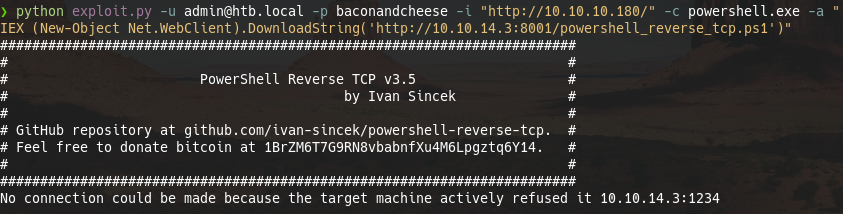
\includegraphics[width=0.9\textwidth]{images/remote/exploit.png}
		\caption{Comando del exploit}
	\end{figure}
	\item Levantamos un servidor en python3 para poder subir el payload al sistema y crear el backdoor.
	\begin{figure}[h]
		\center
		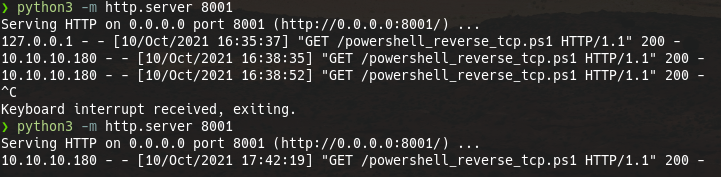
\includegraphics[width=0.9\textwidth]{images/remote/server-python.png}
		\caption{Server de Python3 en escucha}
	\end{figure}
	\item Un payload para establecer la conexión, este lo obtenemos de \textbf{\href{https://github.com/ivan-sincek/powershell-reverse-tcp/blob/master/src/powershell_bind_tcp.ps1}{https://github.com/ivan-sincek/powershell-reverse-tcp.}}.
	\begin{figure}[h]
		\center
		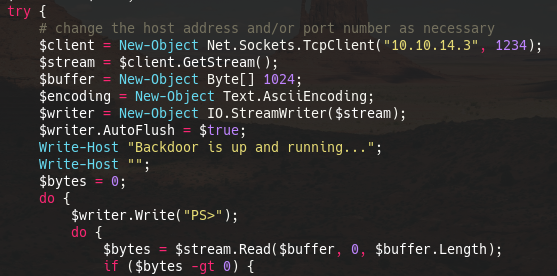
\includegraphics[width=0.9\textwidth]{images/remote/payload.png}
		\caption{Imagen del payload modificado con nuestra dirección}
	\end{figure}
\clearpage
	\item Tener escuchando con netcat un puerto para establecer la conexión por el payload.
	\begin{figure}[h]
		\center
		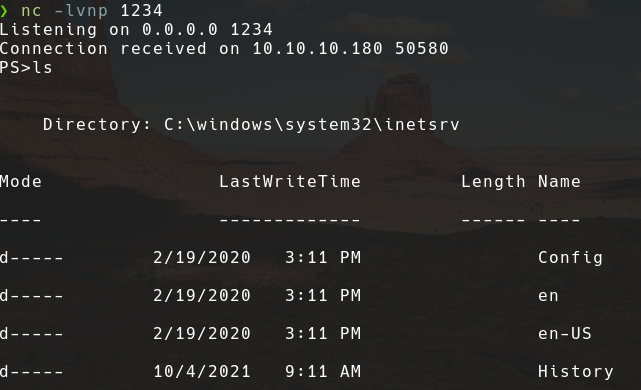
\includegraphics[width=0.78\textwidth]{images/remote/netcat.png}
		\caption{Estableciendo contacto con el netcat}
	\end{figure}
	\item Por último solo quedaría acceder a la carpeta del usuario y abrir el user.txt 
	\begin{figure}[h]
		\center
		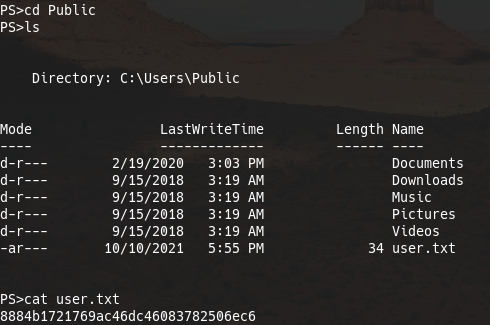
\includegraphics[width=0.78\textwidth]{images/remote/flag-usuario.png}
		\caption{Observando en texto claro la flag}
	\end{figure}

\end{enumerate}

\clearpage

\subsubsection{Escalamiento de Privilegios}
Para el escalamiento de privilegios lo primero que hice fue fijarme en los permisos que tenía con mi usuario actual, esto se puede hacer mediante el comando "whoami /priv".
\begin{figure}[h]
	\center
	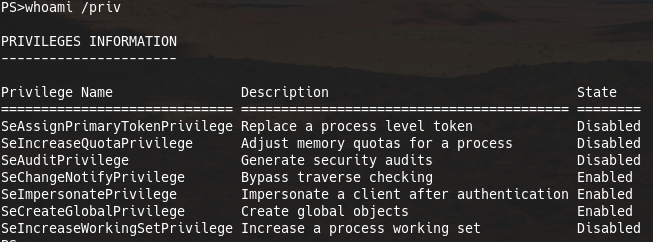
\includegraphics[width=\textwidth]{images/remote/privilegios.png}
	\caption{Verificando Privilegios}
\end{figure}
Luego de esto, había que averiguar la versión del sistema para poder empezar a buscar algún exploit relacionado a los permisos habilitados.
\begin{figure}[h]
	\center
	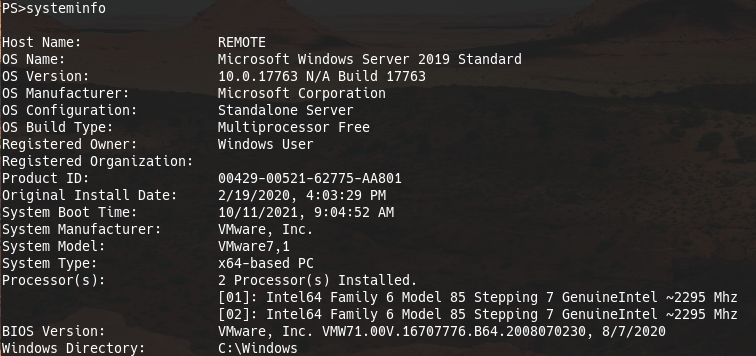
\includegraphics[width=\textwidth]{images/remote/systeminfo.png}
	\caption{Información del Sistema}
\end{figure}

\clearpage

Entonces encontramos un github que hablaba sobre el abuso del permiso \textbf{SeImpersonatePrivilege} en servidores 2016-2019, entonces mediante el script encontrado en : \\ \textbf{\href{https://github.com/itm4n/PrintSpoofer/tree/v1.0}{https://github.com/itm4n/PrintSpoofer/tree/v1.0}} 
\\ Luego de pasar el script a la máquina víctima mediante el uso de un servidor local en python3 y el comando en powershell invoke-webrequest que sirve a modo de wget para obtener una descarga de otro servidor.
el script llamado exploit.exe y el netcat llamado nc.exe son necesarios para poder levantar la reverse shell con permisos elevados.

\begin{figure}[h]
	\center
	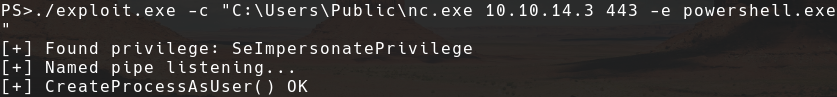
\includegraphics[width=\textwidth]{images/remote/fallo-exploit.png}
	\caption{Ejecutando el script de elevación.}
\end{figure}
Aparentemente funciona pero luego no detecta nada en el puerto de escucha, se hizo una corroboración por md5 a ver si el archivo era exactamente el mismo, pero debido a ciertas circunstancias esta forma no se dejó.
\begin{figure}[h]
	\center
	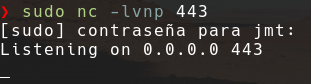
\includegraphics[width=0.4\textwidth]{images/remote/fallo-escucha.png}
	\caption{Fallo en la escucha}
\end{figure}
Entonces al fallar esta forma empecé a ver los procesos del sistema a ver si había alguna pista sobre cómo escalar privilegios, encontré todos los procesos no terminados del exploit que estaban corriendo en background.
y entonces encontré un proceso de TeamViewer7 corriendo.
\begin{figure}[h]
	\center
	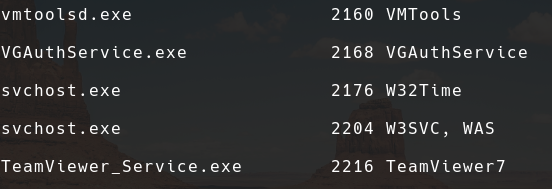
\includegraphics[width=0.7\textwidth]{images/remote/proceso-encontrado.png}
	\caption{Proceso de TeamViewer}
\end{figure}
Buscando un poco sobre algún exploit relacionado a la versión 7, encontré una forma de dumpear las claves de registro que se encuentran en ciertas rutas, un poco más de la documentación se encuentra en : 
\textbf{\href{https://whynotsecurity.com/blog/teamviewer/}{https://whynotsecurity.com/blog/teamviewer/}}

\clearpage

Entonces nos dirigimos a la ruta en cuestión para poder dumpear la clave de registro.
\begin{figure}[h]
	\center 
	\includegraphics[width=0.7\textwidth]{images/remote/confirmación-hash.png}
	\caption{Verificando llave disponible}
\end{figure}

Ya averiguamos de qué parámetro tenemos que buscar la llave, googleando un poco encontramos la ruta y es la siguiente, entonces solo tocaría dumpear.
\begin{figure}[h]
	\center 
	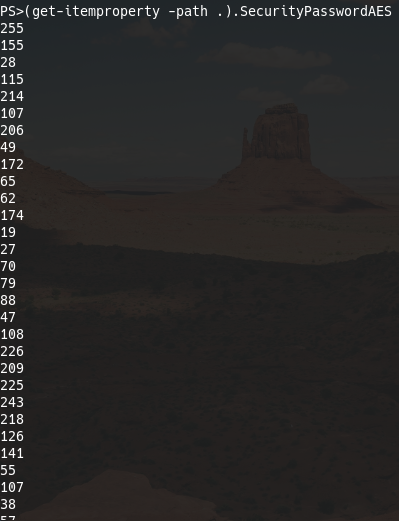
\includegraphics[width=0.43\textwidth]{images/remote/dumpeo-hash.png}
	\caption{Dumpeando la clave}
\end{figure}

\clearpage

Ahora lo que sigue es crackear esta contraseña, según vimos en la vulnerabilidad usa un cifrado AES-128-CBC con la llave 0602000000a400005253413100040000, encontré un script que se usaba para dumpear las credenciales de este exploit específicamente y es el siguiente.
\begin{figure}[h]
	\center 
	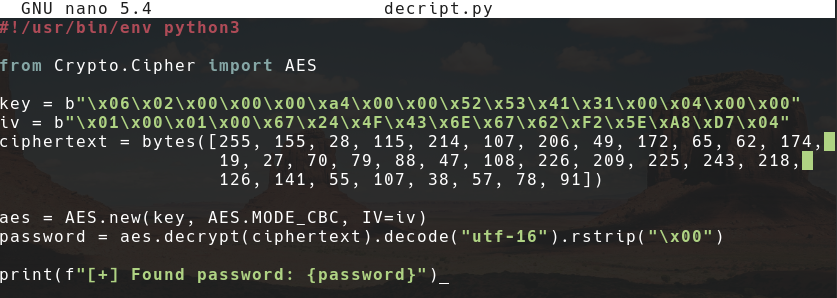
\includegraphics[width=\textwidth]{images/remote/script-python-hash.png}
	\caption{Script de Python para decifrar la clave}
\end{figure}

Con esto obtuvimos la contraseña que era \textbf{!R3m0te!}, ya con esta clave obtenida podemos usar algún impacket para acceder a la máquina, en este caso usamos el psexec.py ubicando el github \textbf{\href{https://github.com/SecureAuthCorp/impacket/blob/master/examples/psexec.py}{https://github.com/SecureAuthCorp/}}.
\begin{figure}[h]
	\center 
	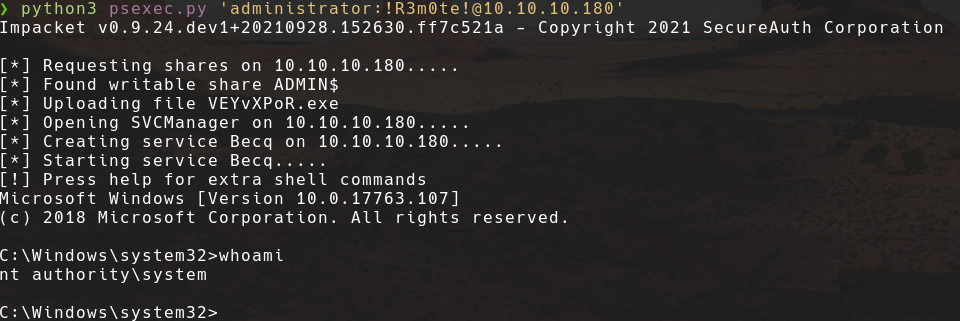
\includegraphics[width=\textwidth]{images/remote/exito-administrator.png}
	\caption{entrando como NT Authority System}
\end{figure}

Con esto ya podríamos obtener la bandera root en C:\textbackslash Users\textbackslash Administrator\textbackslash Desktop\textbackslash root.txt.
Y así finalizaría el acceso completo a la máquina Remote, con los máximos privilegios se puede hacer de todo, así que con esto en mente lo que sigue ahora es la parte de post explotación, en la cual principalmente se hará el hardening de las vulnerabilidades para que no haya problemas críticos en la seguridad.
\clearpage

\subsection{Hardening}

\subsubsection{Umbraco}

Para evitar el ingreso por el vector de umbraco se requiere una actualización, pero debido a que pasar de Umbraco 7 al 8 o 9 no es tan sencillo, gracias a la incompatibilidad de código que hay entre versiones, la única solución que quedaría sería netamente pasar el contenido de forma manual de una versión a otra.
Esta es la solución oficial que nos dan en la documentación de Umbraco, sin embargo esta versión es completamente obsoleta así que solo quedaría hacer la migración manual como sugieren.
De hecho gracias a la versión que se tiene en el servidor, que es la 7.12.4, no tiene forma de migrar.
\begin{figure}[h]
	\center 
	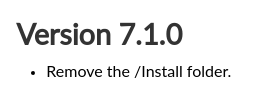
\includegraphics[width=0.3\textwidth]{images/remote/umbraco-version.png}
	\caption{Solución Oficial de Umbraco}
\end{figure}
\\ Entonces la única solución sería instalar una nueva versión de Umbraco 9 y configurar el servidor desde esa base.

\subsubsection{Permisos Powershell}

También se tuvo un problema con los permisos o privilegios que tenía el usuario con el que se escaló privilegios, debido a la versión 2019 de servidor que se usaban era necesario verificar que el permiso \textbf{SeImpersonatePrivilege}-
Para lo cual se tiene que deshabilitar mediante un script referenciado en 


\begin{lstlisting}
	function Add-ServiceLogonRight([string] $Username) {
		Write-Host "Enable ServiceLogonRight for $Username"
	
		$tmp = New-TemporaryFile
		secedit /export /cfg "$tmp.inf" | Out-Null
		(gc -Encoding ascii "$tmp.inf") -replace '^SeServiceLogonRight .+
		', " `$0,$Username" | sc -Encoding ascii "$tmp.inf"
		secedit /import /cfg "$tmp.inf" /db "$tmp.sdb" | Out-Null
		secedit /configure /db "$tmp.sdb" /cfg "$tmp.inf" | Out-Null
		rm $tmp* -ea 0
	}
\end{lstlisting}	

Con esto ya evitaría que se pueda escalar privilegios mediante el exploit en Windows Server 2019.

\subsubsection{TeamViewer7}

Para instalar esto se necesitaría o eliminar el proceso o actualizar la versión a la más nueva, pero desde cmd o powershell no se puede actualizar de forma sencilla los programas debido a la forma en la que están hechos y el funcionamiento de la terminal en windows.
De todos modos se podría actualizar luego de instalar un programa llamado winget ubicado en \textbf{\href{https://github.com/microsoft/winget-cli/releases}{https://github.com/microsoft/winget-cli/releases}}


\clearpage
% ----------------------------FUSE-----------------------------------
\section{Fuse}
\subsection{Reconocimiento}
\subsection{Escaneo de Vulnerabilidades}
\subsection{Enumeración}
\subsection{Explotación}
\subsection{Post Explotación}

\end{document}
